\section{Скирмион}
Для получения визуального представления скирмиона положим коэффициент
диссипации $\gamma=0$. Спины в изначальной конфигурации поля направим по
направлению магнитного поля кроме одного, направленного в противоположную
сторону, получается рисунки следующего вида~\ref{fig:skyrmion}.

\begin{figure}[H]
    \centering
    \begin{subfigure}[b]{0.49\textwidth}
        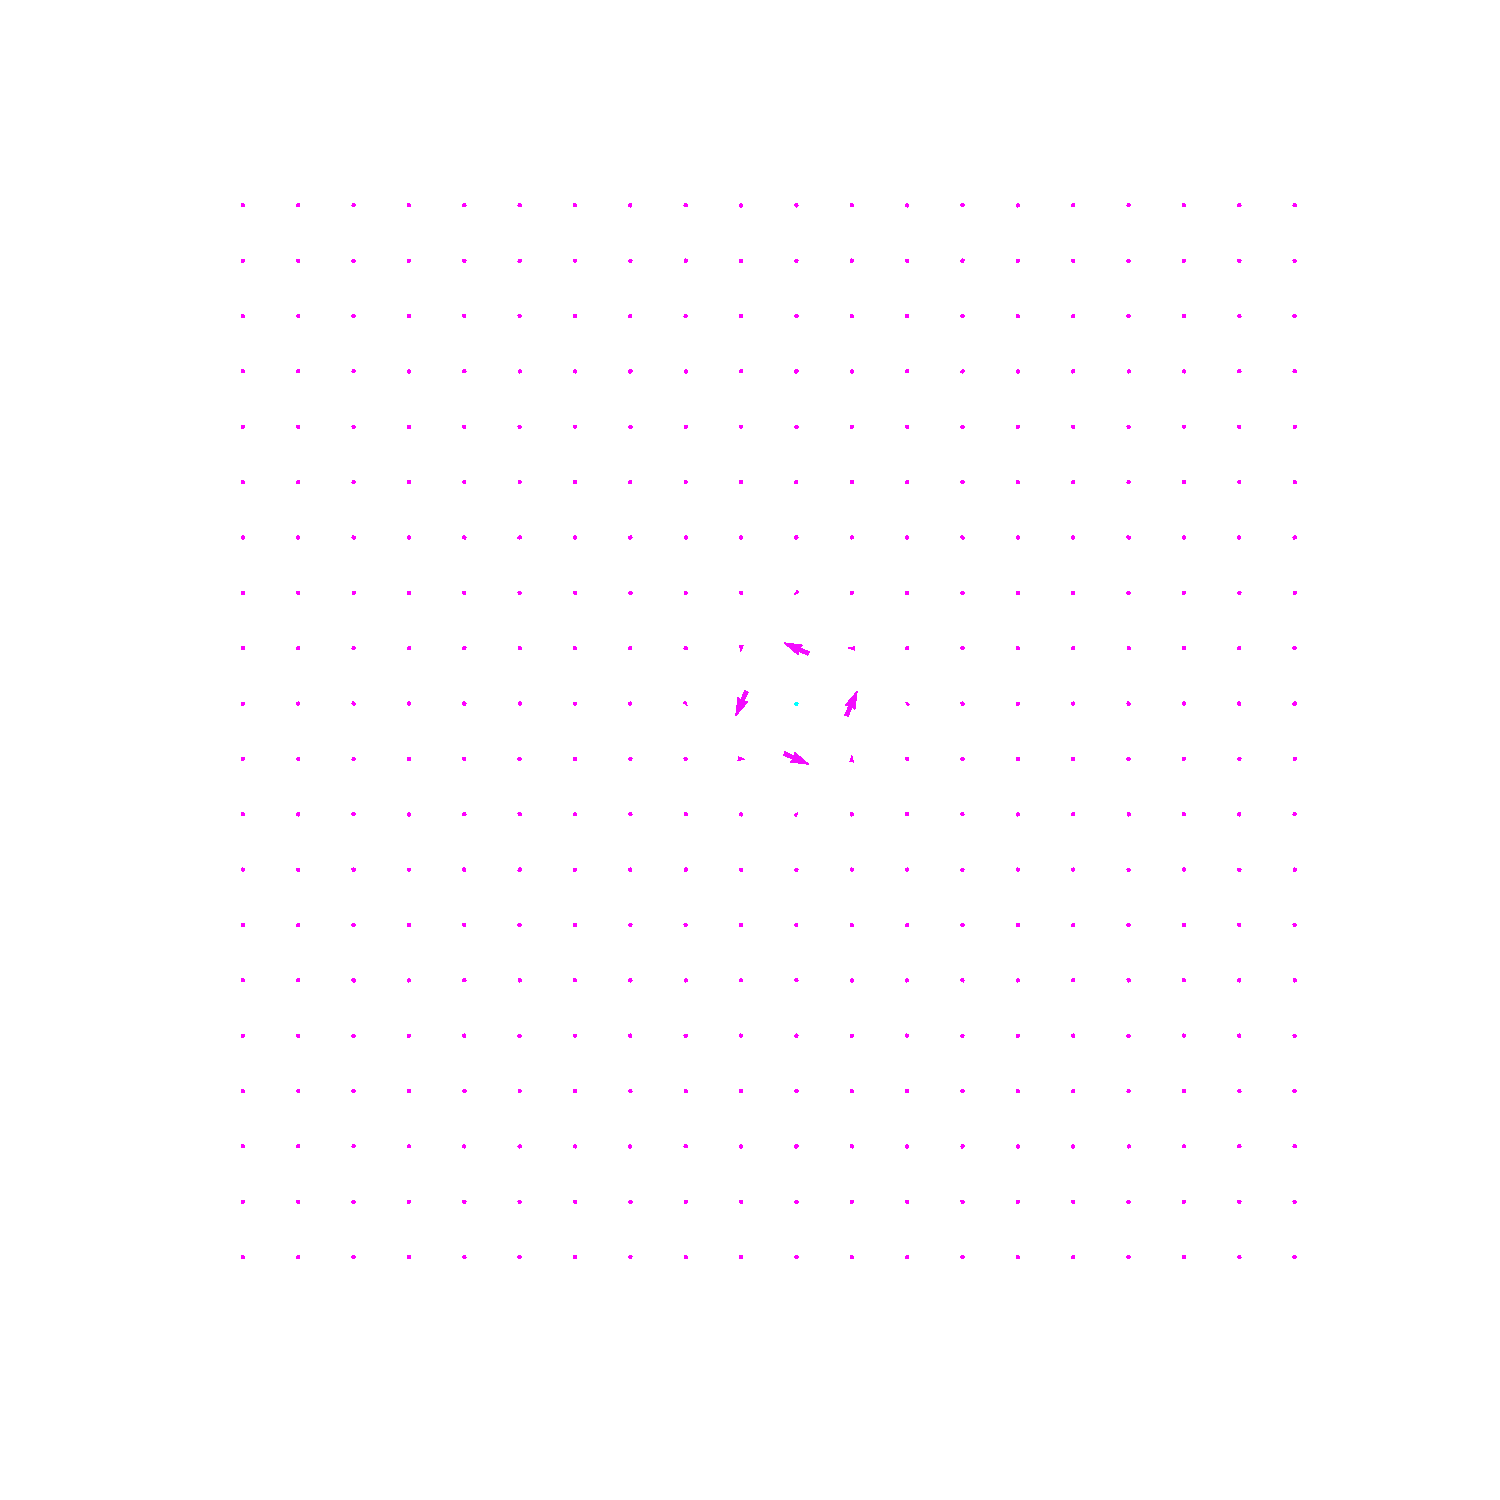
\includegraphics[width=\textwidth]{skyrmion1.pdf}
    \end{subfigure}
    \begin{subfigure}[b]{0.49\textwidth}
        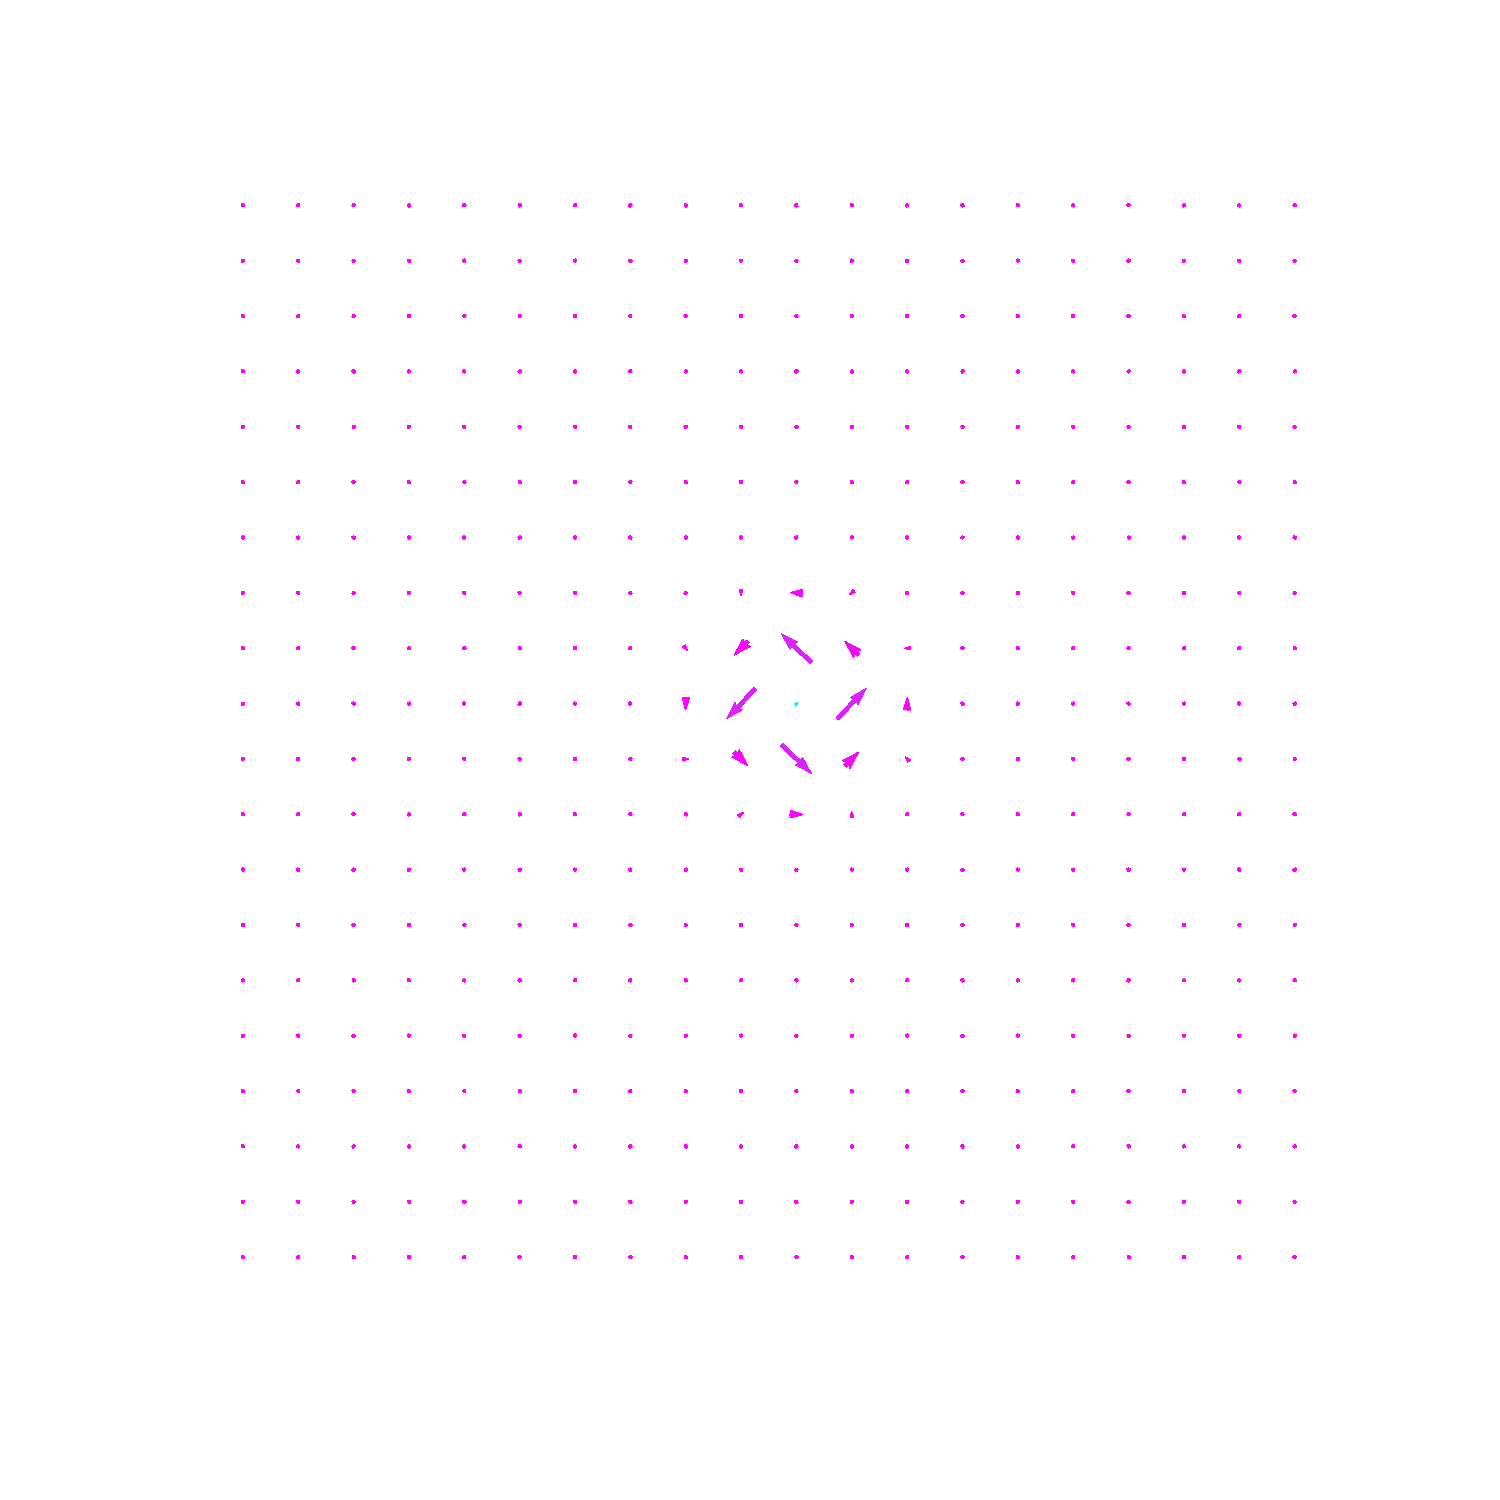
\includegraphics[width=\textwidth]{skyrmion2.pdf}
    \end{subfigure}
    \begin{subfigure}[b]{0.49\textwidth}
        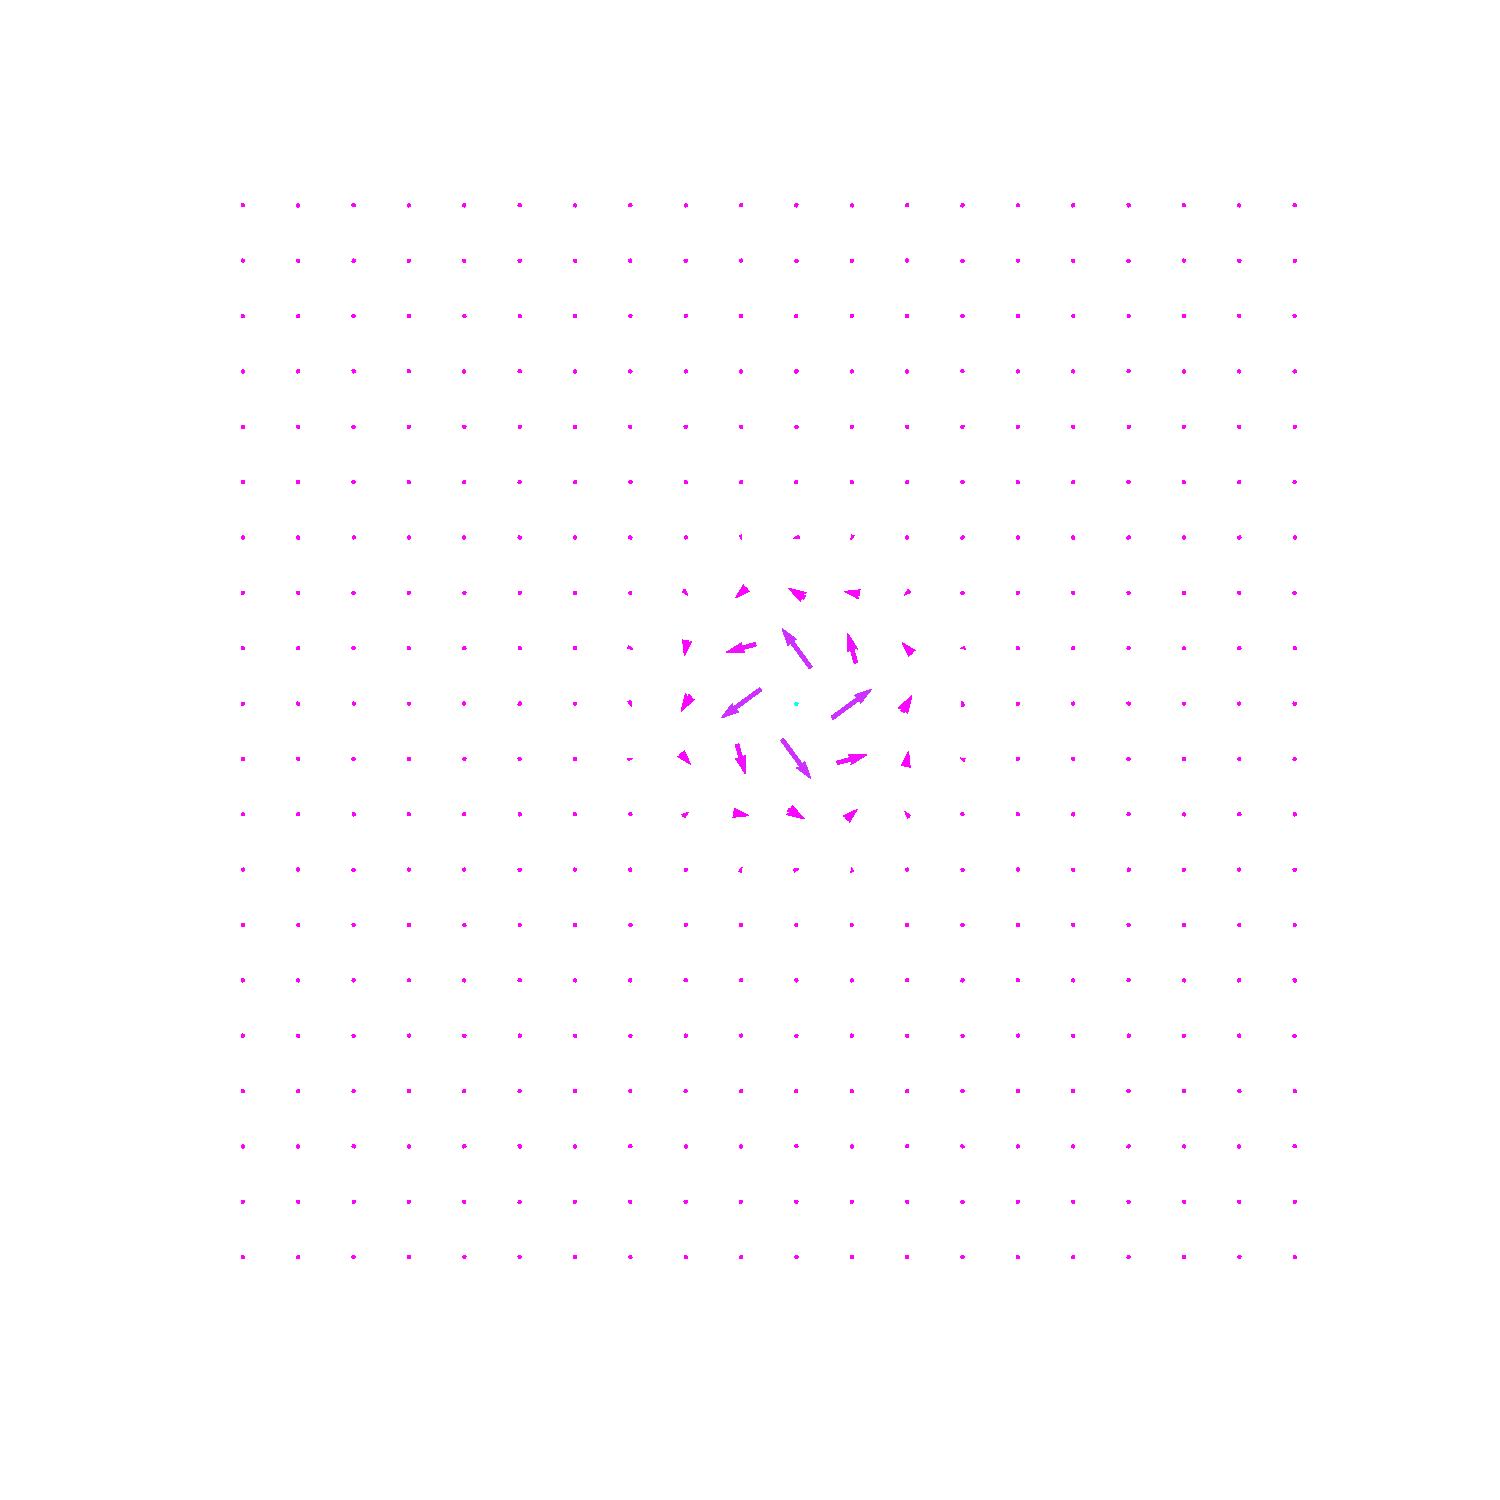
\includegraphics[width=\textwidth]{skyrmion3.pdf}
    \end{subfigure}
    \begin{subfigure}[b]{0.49\textwidth}
        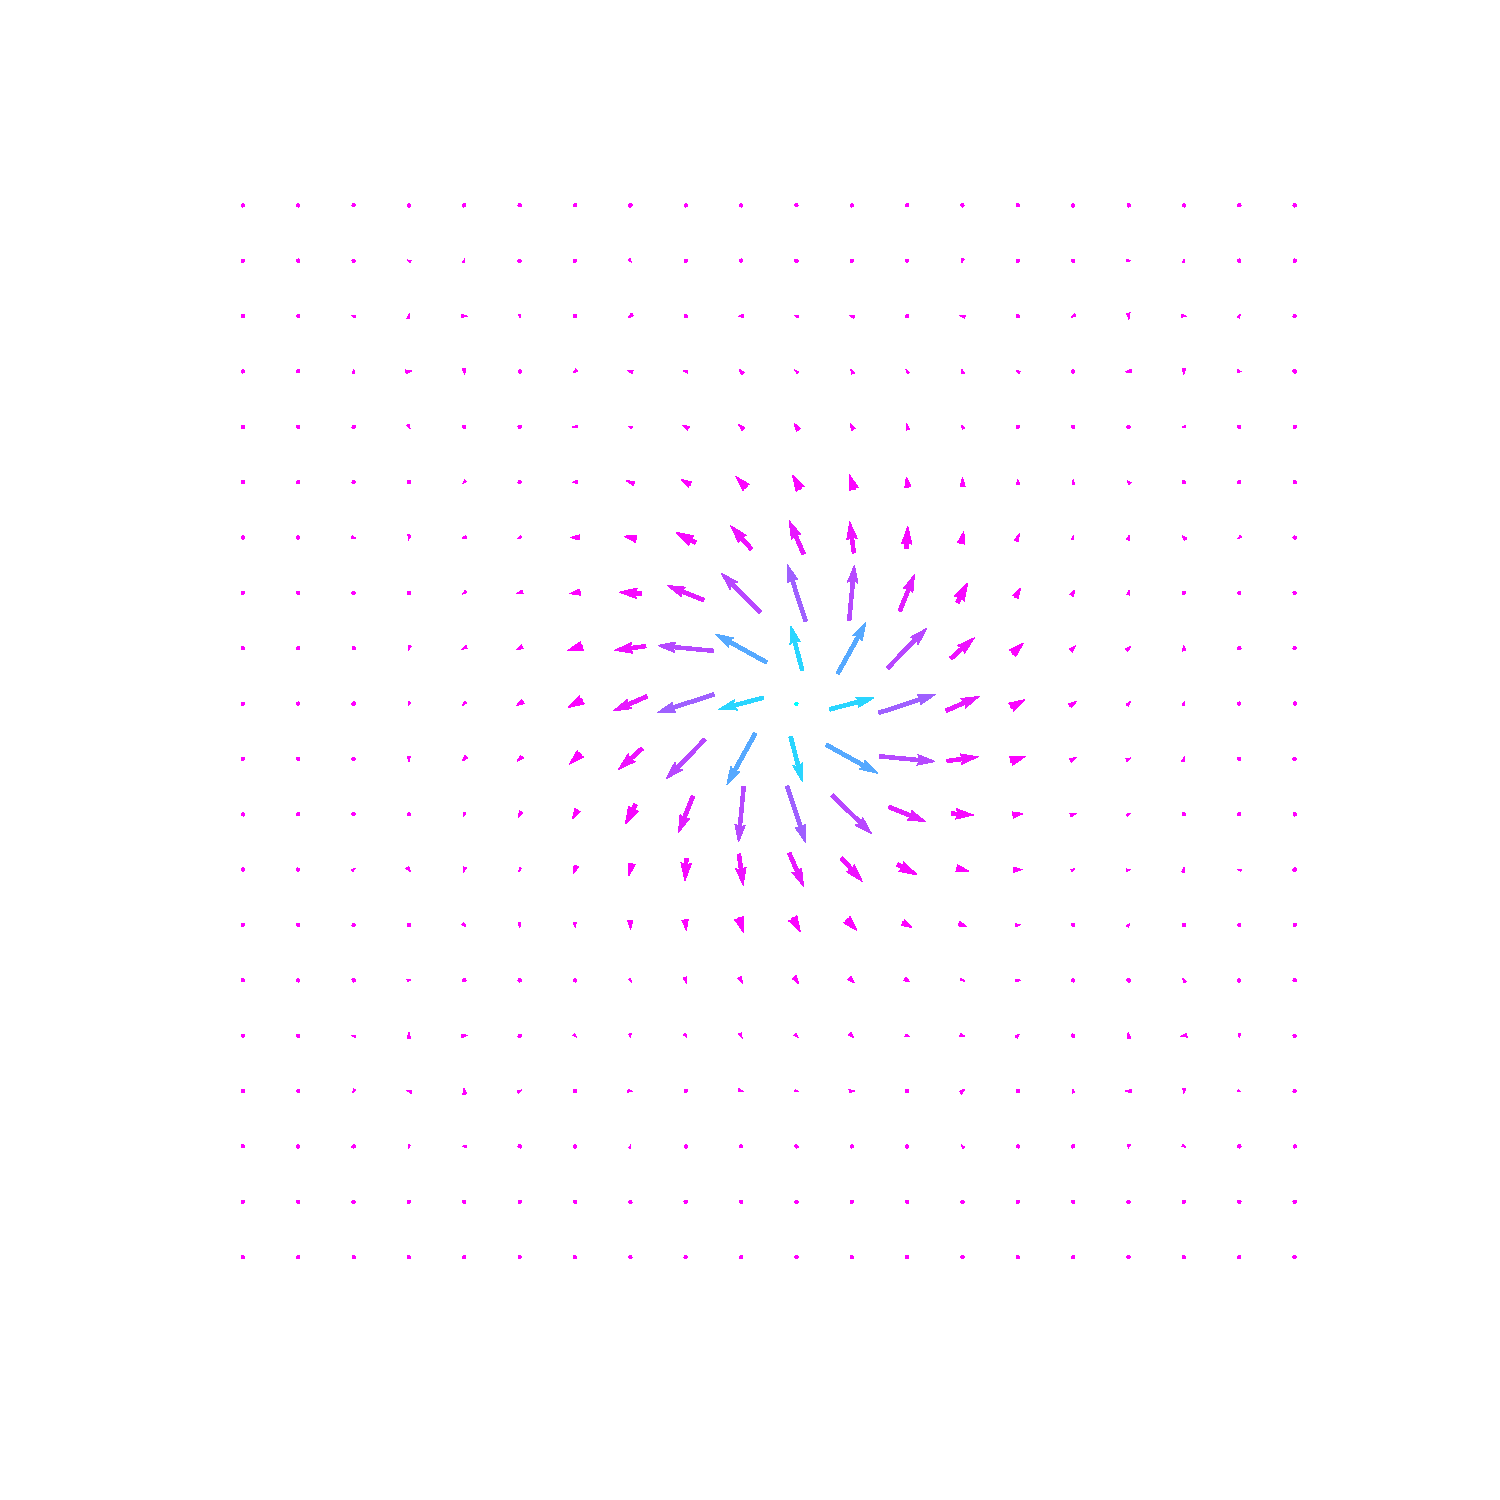
\includegraphics[width=\textwidth]{skyrmion4.pdf}
    \end{subfigure}
    \caption{Различные стадии скирмиона.}
\label{fig:skyrmion}
\end{figure}
